%(BEGIN_QUESTION)
% Copyright 2011, Tony R. Kuphaldt, released under the Creative Commons Attribution License (v 1.0)
% This means you may do almost anything with this work of mine, so long as you give me proper credit

Lag et regneark som beregner bredden på en \textit{Fresnel-sone} mellom to antenner, gitt frekvens, signalbaneavstand, posisjon målt fra den ene antennen og Fresnel-sonenummer. Et eksempeloppsett vises her, der gult markerer verdier som skal tastes inn, og blått markerer verdier som regnearket beregner:

$$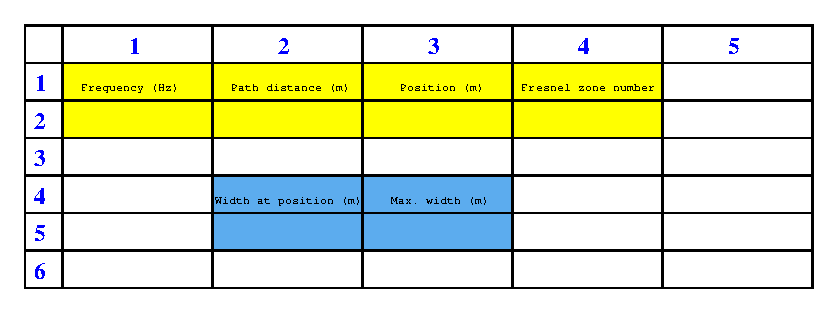
\includegraphics[width=15.5cm]{i00332x01.eps}$$

\vskip 20pt \vbox{\hrule \hbox{\strut \vrule{} {\bf Forslag til sokratisk diskusjon} \vrule} \hrule}

\begin{itemize}
\item{} Forklar hvordan du kan \textit{teste} det ferdige regnearket for å se at det beregner Fresnel-sonebredde korrekt.
\item{} Hvis vi er opptatt av at Fresnel-sonen skal klarere området mellom to parallelle trær på hver side av siktlinjen, må vi beregne \textit{radius} eller \textit{diameter}?
\item{} Hvis vi er opptatt av at Fresnel-sonen skal klarere bakken, må vi beregne \textit{radius} eller \textit{diameter}?
\end{itemize}

\underbar{file i00332}
%(END_QUESTION)





%(BEGIN_ANSWER)


%(END_ANSWER)





%(BEGIN_NOTES)


%INDEX% Computer spreadsheet exercise: Fresnel zone width calculator
%INDEX% Electronics review, Fresnel zones for radio links

%(END_NOTES)
